\documentclass[12pt]{article}
\setlength\headheight{14.5pt}
\title{Homework}
\author{Frederick Robinson}
\date{23 November 2009}
\usepackage{amsfonts}
\usepackage{amsthm}
\usepackage{graphicx}
\usepackage{fancyhdr}
\pagestyle{fancyplain}

\begin{document}

\lhead{Frederick Robinson}
\rhead{Math 381: Fourier Analysis}

   \maketitle

\setcounter{tocdepth}{2} 

\tableofcontents

\section{Chapter 5 Section 2.6}

\subsection{Problem 7}
\subsubsection{Question}
Apply the method of images to solve the initial-value problem 
\[u_t=K u_{xx}\ \ \ \ \ t>0,x>0\]
\[u_x(0;t)=0\ \ \ \ \ t>0\] 
\[u(x;0)=\left\{ \begin{array}{ll}1 & 0\leq x \leq L_1\\ 0 & x>L_1\end{array} \right. \]
Show that $u(x;t)=O(t^{-1/2})$ when $t\to\infty$
\subsubsection{Answer}

So we recognize that this is a Neumann boundary condition so the solution is given as in \cite[Page 305]{pinsky} by
\[u(x;t)=\frac{1}{\sqrt{4\pi K t}}\int_0^\infty \left( e^{\frac{-(x-\xi)^2}{4 K t}}+e^{\frac{-(x+\xi)^2}{4 K t}} \right) f(\xi) d\xi\]
and clearly we can split the domain of integration to
\[u(x;t)=\frac{1}{\sqrt{4\pi K t}} \left( \int_0^{L_1} \left( e^{\frac{-(x-\xi)^2}{4 K t}}+e^{\frac{-(x+\xi)^2}{4 K t}} \right) f(\xi) d\xi +\int_{L_1}^\infty \left( e^{\frac{-(x-\xi)^2}{4 K t}}+e^{\frac{-(x+\xi)^2}{4 K t}} \right) f(\xi) d\xi\ \right) \]
and since $f(\xi)$ is uniformly zero in the second integral and one otherwise we may rewrite this as
\[\frac{1}{\sqrt{4\pi K t}}  \int_0^{L_1} \left( e^{\frac{-(x-\xi)^2}{4 K t}}+e^{\frac{-(x+\xi)^2}{4 K t}} \right)  d\xi   \]

So, we have found the solution to the boundary value problem as desired. Now we will look for some bound for the solution as $x \to \infty$.

But observe that each of ${\frac{-(x-\xi)^2}{4 K t}}$ and ${\frac{-(x+\xi)^2}{4 K t}}$ are negative for $t>0$. Thus, $e^{\frac{-(x-\xi)^2}{4 K t}}$ and $e^{\frac{-(x+\xi)^2}{4 K t}}$ are less or equal to $1$. So, in particular we must have that
\[ \left| \frac{1}{\sqrt{4\pi K t}}  \int_0^{L_1} \left( e^{\frac{-(x-\xi)^2}{4 K t}}+e^{\frac{-(x+\xi)^2}{4 K t}} \right)  d\xi \right| = |u(x;t)| \leq  \frac{1}{\sqrt{4\pi K t}}  \int_0^{L_1} \left(2\right)  d\xi  = \frac{L_1}{\sqrt{\pi K t}}\]
So, $u(x;t)=O(t^{-1/2})$ when $t\to\infty$ as desired.

\subsection{Problem 11}
\subsubsection{Question}

Consider the following initial-value problem for a heat equation with a linear source term:
\[u_t=K u_{xx} +au\ \ \ \ t>0,-\infty<x<\infty\]
\[u(x;0)=f(x)\]
where $a$ is a positive constant that represents the strength of the source term, per unit of temperature.

(a) Find a Fourier representation of the solution

(b) Find an explicit representation of the solution corresponding to the Gauss-Weierstrass integral (5.2.10).

\subsubsection{Answer}

So we will look for solutions as Fourier series in analogy to the process used to determine the solution to such equations without a source term in 5.2.2 \cite[Page 295]{pinsky}. So, let $U(\mu;t)$ be the Fourier transform of $u(x;t)$. So, from the definition of a Fourier transform we have 
\begin{equation}\label{reverse}u(x;t)=\int_{-\infty}^\infty U(\mu;t) e^{i \mu x}d\mu\end{equation}
and
\begin{equation}\label{forwards}U(\mu;t)=\frac{1}{2\pi}\int_{-\infty}^\infty u(x;t) e^{-i \mu x}dx\end{equation}

Now we shall assume that derivatives can be taken under the integral signs to obtain 
\[u_t(x;t)=\int_{-\infty}^\infty U_t(\mu;t) e^{i \mu x} d\mu\]
\[u_x(x;t)=\int_{-\infty}^\infty U(\mu;t) i \mu e^{i \mu x} d\mu\]
\[u_{xx}(x;t)=\int_{-\infty}^\infty U(\mu;t) (i\mu)^2 e^{i \mu x} d\mu\]
so, in order to satisfy the given heat equation we must have
\[0=u_t-Ku_{xx}-au=\int_{-\infty}^\infty \left( U_t + K U\mu^2 -aU \right) e^{i \mu x} d\mu\]
Thus, $U$ must satisfy the ordinary differential equation 
\begin{equation}\label{ode}0=U_t+K\mu^2U-aU=U_t+(K\mu^2-a)U\end{equation}
We may determine the initial conditions for this ODE by taking $t=0$ in Equation \ref{reverse}. So, $U(\mu;0)$ must be given by the Fourier transform of the initial condition $f$ for the original problem, that is
\[U(\mu;0)=F(\mu)\]
Where $F(\mu)$ is the Fourier transform of $f$.

So, our solution to Equation \ref{ode} is given by 
\[U(\mu;t)=F(\mu)e^{(-K\mu^2+a)t}\]
Now we can just substitute this into Equation \ref{reverse} in order to recover the solution we want. We have in particular
\[u(x;t)=\int_{-\infty}^\infty U(\mu;t)e^{i \mu x} d\mu \]
\[=\int_{-\infty}^\infty F(\mu) e^{i\mu x}e^{(a-K \mu^2)t}d\mu \]

Now, it remains only to compute an explicit representation of the solution corresponding to the Gauss-Weierstrass integral. We have 
\[u(x;t)=\int_{-\infty}^\infty F(\mu) e^{i\mu x}e^{(a-K \mu^2)t}d\mu \]
But note that this is just the product of $F$ the Fourier transform of $f$ with $e^{(a-K\mu^2)t}$. Furthermore we know that
\[\int_{-\infty}^\infty e^{i\mu(x-\xi)}e^{(a-k\mu^2)t}d\mu=2\pi \left( \frac{e^{at-\frac{(x-\xi)^2}{4Kt}}}{\sqrt{4 K t \pi}} \right) \]
and so, employing convolution properties of the Fourier tranform \cite[Theorem 5.2]{pinsky} we get the explicit solution:
\[u(x;t)=\int_{-\infty}^\infty f(\xi) \left( \frac{e^{at-\frac{(x-\xi)^2}{4Kt}}}{\sqrt{4 K t \pi}} \right) d \xi \]
as desired.

\subsection{Problem 15}
\subsubsection{Question}

Solve the heat equation $u_t=Ku_{xx}$ with the initial conditions $u(x;0)=T_1$ if $x<0$ and $u(x;0)=0$ if $x>0$. Show that the level curves $u(x;t)=C$ are parabolas passing through $(0,0)$ in the $(x,t)$ plane. Plot these level curves if $K=\frac{1}{2}$, $T_1=100$ for the values $C=10$, $C=30$, $C=50$.

\subsubsection{Answer}

The solution to the heat equation on an infinite rod with no source term is given \cite[Page 297]{pinsky} by
\[u(x;t)=\int_{-\infty}^\infty f(\xi) \frac{e^{-(x-\xi)^2/4 K t}}{\sqrt{4 \pi K t}} d\xi\]
and so, since we have that 
\[f= \left\{ \begin{array}{cc} T_1 & x<0 \\ 0 & x>0\end{array} \right. \]
this just becomes 
\[u(x;t)= \frac{T_1}{\sqrt{4 \pi K t}} \int_{-\infty}^0  e^{-(x-\xi)^2/4 K t} d\xi\]
integrating yields
\[u(x;t)=T_1\left(1-\Phi \left( \frac{x}{\sqrt{2 K t}} \right) \right) \]
just as in Example 5.2.3 \cite[Page 301]{pinsky}. 

Now, we examine level curves of $u(x;t)$. These take the form
\[u(x;t)=C=T_1\left(1-\Phi \left( \frac{x}{\sqrt{2 K t}} \right) \right) \]
for some constant $C$. So we must have
\[1- \frac{C}{T_1}=\Phi \left( \frac{x}{\sqrt{2 K t}} \right)  \]
\[\Phi ^{-1} \left (1- \frac{C}{T_1} \right)=  \frac{x}{\sqrt{2 K t}}   \]
but since for constant $  1- \frac{C}{T_1}  $ we have that $\Phi^{-1} \left (1- \frac{C}{T_1} \right)$ is just some constant (call it $L$) this is just the equation for a parabola through the origin in the $(x, t)$ plane given by 
\[2 K L^2 t = x^2\]

Figures 1-3 are plots of $x$ as a function of $t$ for fixed values of $K$, $T_1$, $C$.

   \begin{figure}
      \centering
      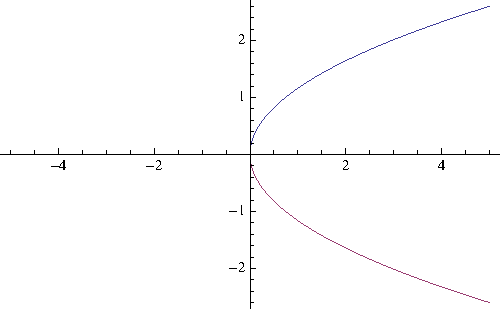
\includegraphics{c10.pdf}
      \caption{$K= \frac{1}{2}$, $T_1=100$, $C=10$}
   \end{figure}

   \begin{figure}
      \centering
      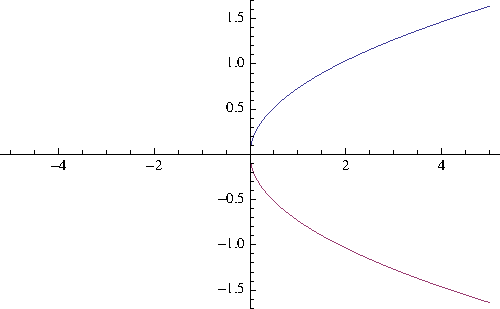
\includegraphics{c30.pdf}
      \caption{$K= \frac{1}{2}$, $T_1=100$, $C=30$}
   \end{figure}

   \begin{figure}
      \centering
      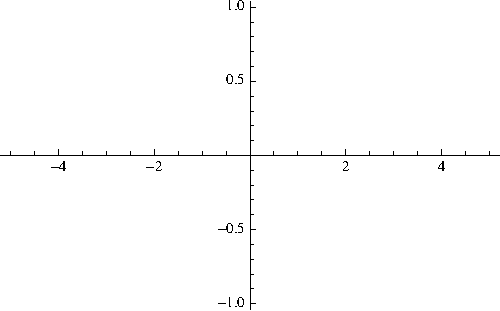
\includegraphics{c100.pdf}
      \caption{$K= \frac{1}{2}$, $T_1=100$, $C=100$}
   \end{figure}


\subsection{Problem 17}
\subsubsection{Question}

Solve the heat equation $u_t=K u_{xx}$ with the initial condititions $u(x;0)=T_1$ if $-L<x<0$, $u(x;0)=T_2$ if $0<x<L$, and $u(x;0)=0$ if $|x|>L$. What is $\lim_{t \to \infty}u(x;t)$?

\subsubsection{Answer}

The solution to the heat equation on an infinite rod with no source term is given \cite[Page 297]{pinsky} by
\[u(x;t)=\int_{-\infty}^\infty f(\xi) \frac{e^{-(x-\xi)^2/4 K t}}{\sqrt{4 \pi K t}} d\xi\]
so, splitting the integral appropriately and employing our particular initial condition we get 
\[u(x;t)=T_1 \int_{-L}^0  \frac{e^{-(x-\xi)^2/4 K t}}{\sqrt{4 \pi K t}} d\xi+T_2 \int_{0}^L \frac{e^{-(x-\xi)^2/4 K t}}{\sqrt{4 \pi K t}} d\xi \]
integrating we get
\[u(x;t)=T_1 \int_{-L}^0  \frac{e^{-(x-\xi)^2/4 K t}}{\sqrt{4 \pi K t}} d\xi+T_2 \int_{0}^L \frac{e^{-(x-\xi)^2/4 K t}}{\sqrt{4 \pi K t}} d\xi \]
\[=T_1 \left( \Phi \left( \frac{x+L}{\sqrt{2 K t}} \right) - \Phi \left( \frac{x}{\sqrt{2 K t}} \right) \right) + T_2 \left( \Phi \left( \frac{x}{\sqrt{2 K t}} \right) - \Phi \left( \frac{x-L}{\sqrt{2 K t}} \right) \right)\]

In the limit when $t \to \infty$ this expression goes to
\[u(x;t)=T_1 \left( \Phi \left( 0 \right) - \Phi \left( 0 \right) \right) + T_2 \left( \Phi \left( 0 \right) - \Phi \left( 0 \right) \right) = 0\]
as we would expect.


\section{Chapter 5 Section 2.8}

\subsection{Problem 1}
\subsubsection{Question}

Use the generating function for Hermite polynomials to prove the equations $H'_k(x)=kH_{k-1}(x), k=1,2,\dots$

\subsubsection{Answer}

\begin{proof}The generating function for Hermite polynomials is 
\[e^{t x -t^2/2}= \sum_{k=0}^\infty \frac{t^k}{k!} H_k(x)=H_0(x)+t H_1(x) +
\frac{t^2}{2} H_2(x) + \dots \] 

So, 


\[\frac{d}{dx}  e^{tx-t^2/2}= t e^{tx-t^2/2} \]
and
\[\frac{d}{dx} \sum_{k=0}^\infty \frac{t^k}{k!} H_k(x) =\sum_{k=0}^\infty \frac{t^k}{k!} H'_k(x) \]
thus
\[t\sum_{k=0}^\infty \frac{t^k}{k!} H_k(x) =\sum_{k=0}^\infty \frac{t^k}{k!} H'_k(x) \]
\[\Rightarrow \sum_{k=0}^\infty \frac{t^{k+1}}{k!} H_k(x) =\sum_{k=0}^\infty \frac{t^k}{k!} H'_k(x) \]
equating like terms we get
\[H'_k(x)=kH_{k-1}(x), k=1,2,\dots\]
as desired.
\end{proof}

\subsection{Problem 3}
\subsubsection{Question}

Combine the results of the two previous exercises to prove the following differential equation satisfied by the Hermite polynomials: $H''_k(x)-xH'_k=-kH_k(x), k=0,1,2,\dots$

\subsubsection{Answer}

First we use the first exercise to get 
\[H'_k(x)=kH_{k-1}(x)\]
\[\Rightarrow H''_k=kH'_{k-1}\]
then, rewriting the result of the second exercise as
\[k H_{k-1}=xH_k-H_{k+1}\]
we can apply it to what we have already to yield
\[H_k''=xH'_k-H'_{k+1}\]
finally, applying the result of the first exercise to the last term we get
\[H_k''=xH'_k-kH_{k}\]
rearranging terms we get
\[H''_k(x)-xH'_k=-kH_k(x)\]
as desired.


\subsection{Problem 5}
\subsubsection{Question}

Use Exercise 3 to show that the functions $\psi_k(x)=e^{-x^2/4}H_k(x)$ satisfy the differential equation $\psi''_k (x)-(x^2/4)\psi_k (x) = -(k+\frac{1}{2} ) \psi_k (x)$ for $k=1,2,\dots$

\subsubsection{Answer}

First we use the definition of $\psi(x)$ to compute some of its derivatives
\[\psi_k'=e^{-x^2/4}H'_k-\frac{1}{2}xe^{-x^2/4}H_k\]
\[\psi_k''=e^{-x^2/4}H''_k-xe^{-x^2/4}H'_k- \left( \frac{1}{2}e^{-x^2/4}-\frac{1}{4}e^{-x^2/4}x^2 \right) H_k\]
so we see that 
\[\psi_k''-(x^2/4)\psi_k=e^{-x^2/4}H''_k-xe^{-x^2/4}H'_k- e^{-x^2/4}\left( \frac{1}{2}-\frac{1}{4}x^2+x^2/4 \right) H_k\]
\[=e^{-x^2/4}H''_k-xe^{-x^2/4}H'_k- \left( \frac{1}{2}e^{-x^2/4}\right) H_k\]
\[=e^{-x^2/4}H''_k-xe^{-x^2/4}H'_k- \frac{1}{2}e^{-x^2/4}  H_k\]
Employing the result from the previous exercise we get
\[=e^{-x^2/4}\left( H''_k-x H'_k- \frac{1}{2}  H_k \right)\]
\[=e^{-x^2/4}\left(-kH_k- \frac{1}{2}  H_k \right)\]
\[=e^{-x^2/4} H_k \left(-k- \frac{1}{2}  \right)\]
\[=- \psi_k \left(k+ \frac{1}{2}  \right)\]
But this is what we wanted to prove.



\section{Chapter 5 Section 3}

\subsection{Problem 1}
\subsubsection{Question}

Use d'Alembert's formula to solve the wave equation $y_{tt}=c^2y_{xx}$ with the initial conditions $y(x;0)=3\sin{2x}$, $y_t(x;0)=0$.

\subsubsection{Answer}

D'Alembert's formula \cite[Page 320]{pinsky} states
\[y(x; t)=\frac{1}{2}\left(f_1(x+ct)+f_1(x-ct) \right) + \frac{1}{2c} \int_{x-ct}^{x+ct}f_2(\xi) d\xi \]
In our case we have $f_1(x)=3 \sin{2x}$ and $f_2(x)=0$. Thus, substituting into the formula we arrive at 
\[y(x; t)=\frac{3}{2}\left( \sin{(2x+2ct)}+\sin{(2x-2ct)} \right)   \]
Now we may employ the trigonometric identity
\[\sin{(\alpha+\beta)}=\sin{\alpha}\cos{\beta}+\cos{\alpha}\sin{\beta}\]
together with the oddness of $\sin{}$ to arrive at
\[y(x; t)=3\sin{2x}\cos{2ct}\]

\subsection{Problem 3}
\subsubsection{Question}

Suppose that $f_1$ has two continuous derivatives and $f_2$ has one continuous derivative. Show that (5.3.7) is a solution of the initial-value  problem (5.3.1).

\subsubsection{Answer}


So, in particular we must show that 
\[y(x; t)=\frac{1}{2}\left(f_1(x+ct)+f_1(x-ct) \right) + \frac{1}{2c} \int_{x-ct}^{x+ct}f_2(\xi) d\xi \]
is a solution to the initial value problem 
\[y_{tt}=c^2y_{xx}\]
\[y(x;0)=f_1(x)\]
\[y_t(x;0)=f_2(x)\]
\[-\infty<x<\infty\ \ \ t>0\]

First we verify that the solution satisfies the wave equation.
\[y_{tt}=\frac{c^2}{2}\left(f''_1(x+ct)+ f''_1(x-ct) \right) + \frac{c}{2} \left( f'_2(x+ct)-f'_2(x-ct)  \right) \]
Moreover,
\[y_{xx}=\frac{1}{2}\left(f''_1(x+ct)+ f''_1(x-ct) \right) + \frac{1}{2c} \left( f'_2(x+ct)-f'_2(x-ct)  \right) \]
so we see that $y_{tt}=c^2y_{xx}$ as desired. Now we check to make sure that our solution satisfies the initial conditions.
\[y(x;0)=\frac{1}{2}\left(f_1(x)+f_1(x) \right) + \frac{1}{2c} \int_{x}^{x}f_2(\xi) d\xi \]
\[=f_1(x)  \]
as desired. Also,
\[y_t(x; t)= \frac{c}{2} \left( f'_1(x+ct) - f'_1(x-ct) \right) + \frac{1}{2} \left( f_2(x+ct) + f_2(x-ct) \right) \]
\[ \Rightarrow y_t(x;0)=  f_2(x) \]
as desired. Thus, we have verified that 5.3.7 is a solution for 5.3.1 as desired.





\subsection{Problem 5}
\subsubsection{Question}

Find the solution of the wave equation $y_{tt}=c^2 y_{xx}$ for $t>0$, $x>0$ satisfying the boundary conditions $y(0;t)=s(t)$ and the initial conditions  $y(x;0)=0$, $y_t(x;0)=g(x)$.

\subsubsection{Answer}

We follow the method outlined in \cite[Example 5.3.1 Page 323]{pinsky}. So we look for $y$ in the form $y(x;t)=f(x+ct)+h(x-ct)$. Substituting the initial conditions and boundary conditions this implies in particular that
\begin{equation}\label{1}y(0;t)=s(t)=f(ct)+h(-ct)\end{equation}
\begin{equation}\label{2}y(x;0)=0=f(x)+h(x)\end{equation}
\begin{equation}\label{3}y_t(x;0)=g(x)=c f'(x)-c h'(x)\end{equation}
taking the derivative and rearranging Equation \ref{2} gives us that
\[f'(x)=-h'(x)\]
and employing this together with the Equation \ref{3} we see that
\[g(x)=-c h'(x)-c h'(x)\]
\[g(x)=-2 c h'(x)\]
and now we may take the derivative on both sides yielding
\[\int g(x) dx=-2 c\int h'(x) dx\]
\[\Rightarrow  G(x)  =-2 c  h(x) +K \]
Where $G$ is the antiderivative of $g$ and $K$ is an arbitrary constant.

So since by Equation \ref{2} $f(x)=-h(x) \Rightarrow G(x)  =2 c  f(x) +K $ we have determined both $f$ and $h$. In particular we have
\[f(x)=\frac{G(x)-K}{2 c}\]
\[h(x)=\frac{K-G(x)}{2 c}\]
so, substituting back into the original form of the solution we get
\[y(x;t)=\frac{G(x+ct)-K}{2 c}+\frac{K-G(x-ct)}{2 c}\]
\[=\frac{1}{2c} \left(G(x+ct)-G(x-ct)\right)\]
\[=\frac{1}{2c} \int_{x-ct}^{x+ct} g(\xi) d\xi \]

This is a solution to the initial value problem and holds for $x>ct$. Now we need only incorporate the boundary value defined by Equation \ref{1} to find the solution on the region $0<x \leq ct$. In order to do this examine Equation \ref{1} revealing
\[s(t)-f(ct)=h(-ct)\]
and substitute $t=t-\frac{x}{c}$ to reveal that in particular
\[s(t-\frac{x}{c})-f(ct-x)=h(x-ct)\]
substituting into the form of the solution gives us
\[y(x;t)=f(x+ct)+h(x-ct)\]
\[=f(x+ct)+s(t-\frac{x}{c})-f(ct-x)\]
Now we merely rearrange terms and substitute our $f$ computed above to get
\[\frac{G(x+ct)-K}{2 c}-\frac{G(ct-x)-K}{2 c}+s(t-\frac{x}{c})\]
\[=\frac{1}{2 c}\int_{ct-x}^{x+ct} g(\xi) d\xi+s(t-\frac{x}{c})\]
for $0<x \leq ct$.


\begin{thebibliography}{9}

	\bibitem{pinsky}
	  Mark Pinsky,
	  \emph{Partial Differential Equations and Boundary Value Problems with Applications}.
	  Waveland Press, Illinois,
	  3rd Edition,
	  2003.

\end{thebibliography}


\end{document}
